\documentclass[a4paper, 10pt, english]{article}
%\documentclass[a4paper, 10pt, swedish]{article}

\usepackage[T1]{fontenc}        % Allow for åäö
\usepackage{lmodern}            % Better font for åäö
\usepackage[utf8]{inputenc}     % For åäö in text


\usepackage{babel}              % Language specifics
                                % + hyphenation

\usepackage{subfigure}
\usepackage{amsmath, amssymb}   % Math stuff
\usepackage{gensymb}

\usepackage{graphicx}           % For including graphics
\usepackage{epstopdf}
\bibliographystyle{plain}       % References
%\bibliographystyle{sweplain}    % Swedish references

\usepackage{textcomp}

\usepackage[margin=1in]{geometry}


\usepackage[colorinlistoftodos]{todonotes}					% Todo notes

\usepackage{tikz,pgfplots}
\pgfplotsset{compat=newest}
\pgfplotsset{plot coordinates/math parser=false}

\usepackage{fancyvrb}

\newcommand{\transp}{^\mathsf{T}}
\newlength\figureheight
\newlength\figurewidth


\title{WASP SECC Course: Cloud Module Assignment\\Report}
\author{Kristoffer Bergman, Per Boström, Shervin Parvini Ahmadi}
\date{June, 2017}


\begin{document}
\maketitle

\section{Overview}
This report briefly describes the service created in the Cloud module of the WASP course in Software engineering and cloud computing. 
The task was very time consuming since non of the group members had previous experience from similar work. Nevertheless, a scalable video conversion has been developed and is described in the following.

Git repository for the code is found at: \verb|https://github.com/perbostrm/cloudassignment|.


\begin{figure}
	\label{fig:architecture}
	\centering
	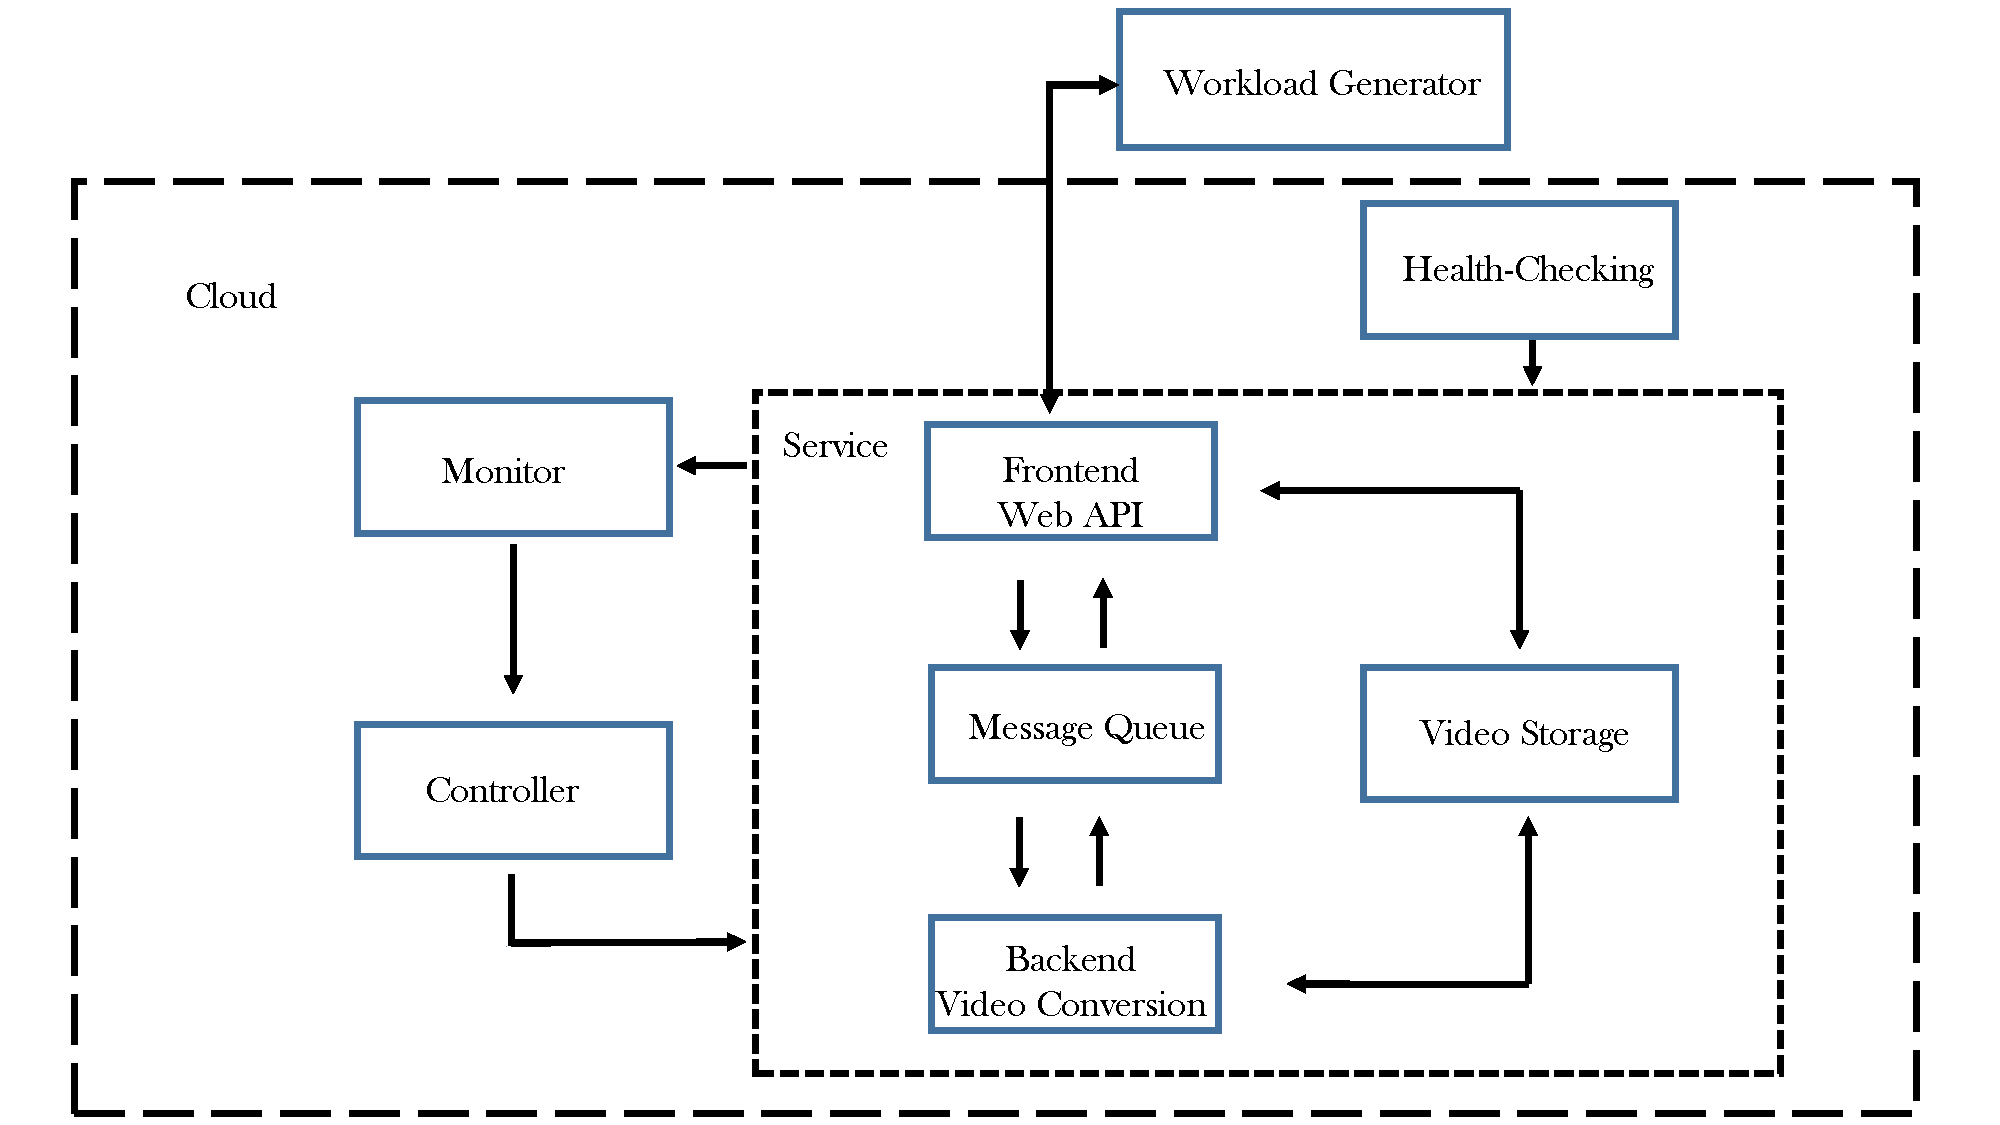
\includegraphics[width=1\textwidth]{figs/workflow-final.pdf}
	\caption{Overview of the system architecture.}
\end{figure}
An overview of the system architecture can be found in Figure~\ref{fig:architecture}. The different components involved are:
\begin{itemize}
	\item \textbf{Workload generator}: Is used as a test engine to simulate external users. See Section~\ref{sec:WG} for more details.
	\item \textbf{Load balancer}: Was not implemented due to lack of time.
	\item \textbf{Frontend Web API}: Is used to receive requests from users and deliver a response. See Section~\ref{sec:FE} for more details.
	\item \textbf{Message queue}: Is used to route the requests to the available Video conversion nodes and maintain the request queue. 
	\item \textbf{Backend Video conversion}: Is used to do the actual conversion of videos by reading the video from the storage. See Section~\ref{sec:BE} for more details.
	\item \textbf{Video Storage}: Is used to store available and converted videos.
	\item \textbf{Monitor}: Is be used to monitor entities relevant for the controller, by periodically gather information. The information is saved in .mat files, which can be used to plot the data in Matlab.
	\item \textbf{Controller}: Is used to make the service scalable. See Section~\ref{sec:Controller} for more details.
	\item \textbf{Health-Checking}: Is used to perform health checking for the backend and frontend nodes.
\end{itemize}

\section{Software and tech}
The following is a list of the software and tech that is used in the system components:
\begin{itemize}
	\item \textbf{Workload generator}: Python
	\item \textbf{Frontend Web API}: Python
	\item \textbf{Message queue}: RabbitMQ
	\item \textbf{Backend Video conversion}: FFmpeg with ffmpy
	\item \textbf{Video Storage}: Object storage in OpenStack
	\item \textbf{Monitor}: Python
	\item \textbf{Controller}: Python with python-novaclient (To interact with OpenStack).
	\item \textbf{Health-Checking}: Python with python-novaclient (To interact with OpenStack)
\end{itemize}

\section{Redundancy}
Due to lack of time, we were unable to implement redundancy in the components with states (such as the Message Queue and the Monitor).

\section{Workload generator} \label{sec:WG}
The workload generator is the test engine that simulates external users. It takes two parameters: the number of client converters and the average time between conversion requests. It starts the specified number of client threads, where each one represents a user. Each user randomly selects a video, sends a conversion request, waits for the completion, and then sleeps for a while (on average the specified time) before repeating the process.

The workload generator also measures the response time and stores it in a .mat-file.

\section{Frontend Web API} \label{sec:FE}
The Frontend Web API is used to receive requests from users and deliver a response. The conversion request is handled according to the following steps
\begin{itemize}
	\item The Frontend Web API receives a video conversion request, and sends this request to the Message Queue.
	\item Then, it waits for a response from the backend, which contains information of how to find the converted video in the storage.
	\item Finally, an "Accepted" response is sent to the user, where the information of how to find the converted video in the storage is included. If the backend does not accept the conversion request, an Error message is returned. 
\end{itemize}
When a user is requesting the actual converted video, the Frontend Web API checks if the converted video (which has a unique name) is available in the Video Storage using python-swiftclient. If it can be found, it responds with a OK message, otherwise an Error messasge is returned.


\section{Backend Video Conversion} \label{sec:BE}
The Backend Video Conversion node is used to perform the actual conversion of videos. When a conversion request is received from the Message Queue, the following steps are executed
\begin{itemize}
	\item First, the node checks if the requested video exists in the folder of available videos. If it does, the node sends an Accepted response back to the queue together with an unique file name, which represent where the converted file will be stored. Otherwise, an Error response is returned and the conversion is aborted. 
	\item The second step is to download the requested video from Video Storage and perform the actual conversion. For this, we used FFmpeg together with a Python wrapper called ffmpy.
	\item Finally, the converted file is uploaded to the Video Storage. Once this is done, the converted and downloaded videos are deleted locally.
\end{itemize}

\section{Controller} \label{sec:Controller}
The controller is used to scale up and down the number of VMs used for backend video conversion, depending on the workload. The controller is running at a frequency of 0.2 Hz

We used the simplifying assumption that all videos are of approximately the same size. This makes it possible to use the time from that a video conversion request is submitted until the video is converted as the control objective. Assume the average time it takes for one core to convert one video is given (including potential delays in the system), and denote it $ T_{\text{conv}} $. With $ n_{\text{queue}} $ video conversion requests in queue and $ n_{\text{vm}} $ active VMs, the time $ T $ needed to convert all videos in the queue is given by
\begin{equation}
T = \frac{T_{\text{conv}}  n_{\text{queue}}}{n_{\text{vm}}}
\end{equation}
Thus, if the control objective is to keep the maximum time from a request is submitted until the video is converted below $ T_{\text{max}} $, the number of VMs needed is given by
\begin{equation}
n_{\text{vm}} > \frac{T_{\text{conv}}  n_{\text{queue}}}{T_{\text{max}}}
\end{equation}

This is of course a simple approach which, if needed, could be extended to also consider videos of varying sizes and possibly reordering the queue such that for example small sized videos are prioritized over larger ones. By some simple tests, we got that $T_{\text{conv}} \approx 4$ seconds when we only had one request running at the time. We used $T_{\text{max}} = 12$ as the maximum , which gave us

\begin{equation*}
	r_{\text{vm}} = \text{max}\{n_{\text{lowest}}, \text{min}\{n_{\text{highest}}, \frac{T_{\text{conv}}  n_{\text{queue}}}{T_{\text{max}}}\} \}
\end{equation*} 
where $n_{\text{lowest}} = 2$ is the lowest amount of  active video conversion nodes, and $n_{\text{highest}} = 10$ is the highest amount of active video conversion nodes. 

To reduce the effect of quick, temporary  changes in the queue, we have used a low-passed filtered reference signal. We have also implemented a minimum time to live for the video conversion nodes, since the time from creation to actual work is long (currently couple of minutes, see Figure~\ref{fig:numberOfVMs}).

\section{Health-Checking} \label{sec:HC}
The Health-Checking node is used to make sure that the available Backend and Frontend nodes works. This is done by checking the Status flag in OpenStack. If a node has status Error, this node is deleted and then re-created again. This is done by using python Novaclient.


\section{Experimental Results}
Since we did not have time to implement the robustness for the system, the experimental evaluations were focused on scaling the service up and down depending on the workload. During the experiments, the workload generator was for convenience executed within the cloud. 

Figures \ref{fig:conversionsPending}--\ref{fig:conversionTime} show data from a scale up and scale down scenario. The sharp increase in workload at $ t=20 $ minutes leads to a substantial increase in the time it takes to handle conversion requests. To handle this, the controller increases the reference and more VMs are created. However, due to long boot times, it takes some time before the new VMs can start working. Also, we noticed that during the startup of new VMs, the ones that were already up and running seemed to slow down. The scaling down is handled in a similar manner; as the workload decreases, fewer VMs are needed and hence some of them are shut down.

\setlength\figureheight{0.21\columnwidth}
\setlength\figurewidth{0.8\columnwidth}
\begin{figure}
	\centering
	% This file was created by matlab2tikz.
%
%The latest updates can be retrieved from
%  http://www.mathworks.com/matlabcentral/fileexchange/22022-matlab2tikz-matlab2tikz
%where you can also make suggestions and rate matlab2tikz.
%
\definecolor{mycolor1}{rgb}{0.89412,0.10196,0.10980}%
%
\begin{tikzpicture}

\begin{axis}[%
width=\figurewidth,
height=\figureheight,
at={(0\figurewidth,0\figureheight)},
scale only axis,
xmin=0,
xmax=60.5651666641235,
xlabel style={font=\color{white!15!black}},
xlabel={Time [minutes]},
ymin=0,
ymax=40,
ylabel style={font=\color{white!15!black}},
ylabel={Conversions pending},
axis background/.style={fill=white},
xmajorgrids,
ymajorgrids
]
\addplot [color=mycolor1, line width=1.2pt, forget plot]
  table[row sep=crcr]{%
0	1\\
0.00800000031789144	0\\
0.139166665077209	1\\
0.20649999777476	2\\
0.316000000635783	3\\
0.335999997456868	2\\
0.408333333333333	1\\
0.434999998410543	0\\
0.604999999205271	3\\
0.649666666984558	2\\
0.805499998728434	3\\
0.847666664918264	3\\
1.07083333333333	4\\
1.10800000031789	3\\
1.1531666636467	2\\
1.20166666507721	1\\
1.30199999809265	1\\
1.46549999713898	4\\
1.48683333396912	3\\
1.57450000047684	2\\
1.60999999841054	1\\
1.70983333190282	2\\
1.92683333158493	3\\
1.9656666636467	3\\
2.22433333396912	4\\
2.28999999761581	3\\
2.33883333206177	2\\
2.56583333015442	4\\
2.6443333307902	3\\
2.96266666650772	4\\
3.10249999761581	3\\
3.30216666460037	3\\
3.44533333381017	3\\
3.61516666412354	3\\
3.79033333063126	4\\
4.04033333063126	4\\
4.09183333317439	3\\
4.31083333094915	3\\
4.42900000015895	3\\
4.64550000031789	3\\
4.73949999809265	4\\
4.81016666491826	4\\
5.10633333126704	4\\
5.19966666698456	3\\
5.43716666698456	3\\
5.53516666491826	4\\
5.91299999952316	4\\
5.97549999952316	3\\
6.08333333333333	2\\
6.22466666698456	4\\
6.30066666603088	4\\
6.48483333190282	3\\
6.59283333222071	4\\
6.84599999984105	4\\
7.05199999809265	3\\
7.17833333015442	3\\
7.24899999698003	2\\
7.33483333190282	2\\
7.46666666666667	2\\
7.60033333301544	2\\
7.68883333206177	2\\
7.99899999698003	4\\
8.05549999872843	3\\
8.24699999888738	4\\
8.34833333094915	3\\
8.75	4\\
8.85099999904633	3\\
8.93949999809265	3\\
9.1068333307902	4\\
9.17699999809265	4\\
9.35233333110809	3\\
9.46183333396912	3\\
9.54299999872844	2\\
9.72233333190282	2\\
9.79899999698003	3\\
10.0306666652362	3\\
10.0794999996821	4\\
10.2513333320618	4\\
10.392666665713	3\\
10.4381666660309	2\\
10.4769999980927	2\\
10.6849999984105	3\\
10.7694999972979	3\\
10.9416666666667	4\\
10.9824999968211	3\\
11.13649999698	3\\
11.276166665554	3\\
11.5308333317439	4\\
11.7241666634878	4\\
11.8091666658719	3\\
11.8889999985695	3\\
11.9708333333333	2\\
12.1883333325386	4\\
12.2593333323797	3\\
12.4604999979337	4\\
12.5556666652362	3\\
12.7794999996821	3\\
12.867666665713	3\\
13.0774999976158	3\\
13.2205000003179	3\\
13.3008333325386	2\\
13.5318333307902	2\\
13.5898333311081	3\\
14.0131666660309	4\\
14.1048333326976	3\\
14.1888333320618	3\\
14.4849999984105	4\\
14.5388333320618	3\\
14.8851666649183	4\\
14.9486666639646	3\\
15.2621666669846	4\\
15.3328333338102	3\\
15.397833331426	2\\
15.5419999996821	2\\
15.5884999990463	1\\
15.9544999996821	4\\
16.0189999977748	3\\
16.3419999996821	4\\
16.3976666649183	3\\
16.6144999980927	4\\
16.7120000004768	3\\
16.8271666646004	4\\
17.0221666653951	4\\
17.093833331267	3\\
17.2834999998411	3\\
17.3294999996821	2\\
17.4336666663488	4\\
17.5828333338102	3\\
17.6408333301544	2\\
18.0163333336512	4\\
18.1503333330154	3\\
18.342666665713	4\\
18.4968333323797	3\\
18.7928333322207	4\\
18.8953333338102	4\\
18.968833331267	3\\
19.3269999980927	4\\
19.4021666646004	3\\
19.6391666650772	3\\
19.7424999992053	3\\
20.0403333306313	4\\
20.1431666652362	3\\
20.5121666669846	2\\
20.5694999972979	1\\
20.6293333331744	0\\
21.1223333319028	39\\
21.2283333301544	38\\
21.3431666652362	39\\
21.4101666649183	38\\
24.322833331426	39\\
24.4120000004768	39\\
24.4804999987284	38\\
24.5344999988874	38\\
24.6126666665077	38\\
24.7006666660309	37\\
24.7963333328565	38\\
24.8569999972979	37\\
24.9359999974569	37\\
25.0268333315849	37\\
25.1366666634878	38\\
25.2634999990463	39\\
25.3658333301544	38\\
25.4399999976158	38\\
25.5533333301544	38\\
25.6314999977748	38\\
25.7673333326976	38\\
25.8983333309491	38\\
26.0324999968211	37\\
26.1533333301544	37\\
26.2766666650772	37\\
26.442666665713	39\\
26.5641666650772	39\\
26.6959999998411	38\\
26.8519999980927	38\\
26.9844999988874	39\\
27.3303333322207	39\\
27.4418333331744	38\\
27.5484999974569	39\\
27.6509999990463	38\\
27.780166665713	37\\
27.8844999988874	37\\
27.9969999988874	38\\
28.0625	38\\
28.5283333301544	39\\
28.5821666638056	38\\
30.5009999990463	39\\
30.6113333304723	38\\
31.2441666642825	39\\
31.3646666646004	39\\
31.451166665554	39\\
31.5101666649183	39\\
31.5611666639646	38\\
31.7291666666667	39\\
31.8216666658719	38\\
31.9156666636467	37\\
31.9879999995232	37\\
32.0671666661898	37\\
32.1378333330154	37\\
32.2211666663488	37\\
32.305166665713	37\\
32.3641666650772	38\\
32.4171666661898	38\\
32.4601666649183	38\\
32.5016666650772	37\\
32.5371666669846	36\\
32.5759999990463	35\\
32.6191666642825	35\\
32.6698333303134	35\\
32.7226666649183	35\\
32.8024999976158	36\\
32.8631666660309	37\\
32.918833331267	38\\
32.9768333315849	38\\
33.0208333333333	38\\
33.0706666668256	37\\
33.1221666653951	36\\
33.1998333334923	38\\
33.2639999985695	37\\
33.3254999995232	37\\
33.3768333315849	38\\
33.4283333301544	38\\
33.4838333328565	38\\
33.5286666671435	37\\
33.5843333323797	37\\
33.635333331426	36\\
33.7076666673024	35\\
33.8336666663488	37\\
33.917666665713	37\\
33.9883333325386	37\\
34.0496666669846	36\\
34.1468333323797	38\\
34.2183333317439	38\\
34.3476666649183	38\\
34.4568333307902	38\\
34.5399999976158	38\\
34.6056666652362	37\\
34.7333333333333	39\\
34.8524999976158	38\\
34.9616666634878	38\\
35.0574999968211	39\\
35.1464999993642	38\\
35.231333331267	38\\
35.3481666644414	38\\
35.4631666660309	39\\
35.5509999990463	38\\
35.6408333301544	37\\
35.7458333333333	39\\
35.8533333301544	38\\
35.92399999698	38\\
35.9796666661898	37\\
36.0344999988874	36\\
36.1076666673024	35\\
36.1866666634877	36\\
36.2581666668256	38\\
36.318833331267	37\\
36.3745000004768	36\\
36.4276666641235	36\\
36.4798333326976	36\\
36.5254999995232	35\\
36.5859999974569	36\\
36.6389999985695	35\\
36.747833331426	38\\
36.8453333338102	37\\
36.9160000006358	36\\
37.0111666639646	37\\
37.0901666641235	37\\
37.1549999992053	36\\
37.2625	36\\
37.3508333325386	36\\
37.4241666634878	37\\
37.5073333303134	37\\
37.5729999979337	36\\
37.6544999996821	37\\
37.781333331267	38\\
37.8653333306313	37\\
37.960333331426	37\\
38.0221666653951	38\\
38.0911666671435	37\\
38.1776666641235	38\\
38.2458333333333	38\\
38.3233333309491	37\\
38.4024999976158	37\\
38.4698333303134	37\\
38.5221666653951	37\\
38.5660000006358	36\\
38.6108333309491	37\\
38.6723333319028	36\\
38.722833331426	37\\
38.7893333315849	37\\
38.8324999968211	37\\
38.8663333336512	36\\
38.9118333339691	36\\
38.9458333333333	37\\
38.9798333326976	36\\
39.0111666639646	35\\
39.0483333309491	35\\
39.0971666653951	34\\
39.1766666650772	36\\
39.2496666669846	37\\
39.3354999979337	38\\
39.3953333338102	38\\
39.4535000006358	37\\
39.5040000001589	36\\
39.5528333306313	37\\
39.6201666673024	38\\
39.7276666641235	37\\
39.8151666641235	37\\
39.8699999968211	39\\
39.9606666644414	38\\
40.0219999988874	37\\
40.0759999990463	36\\
40.1416666666667	37\\
40.2248333334923	37\\
40.3098333319028	37\\
40.3711666663488	37\\
40.4184999982516	36\\
40.5058333317439	36\\
40.5348333319028	36\\
40.5711666663488	35\\
40.6058333317439	34\\
40.6691666642825	35\\
40.7206666668256	35\\
40.763666665554	36\\
40.8026666641235	35\\
40.8686666647593	35\\
40.8991666634878	34\\
40.9278333306313	33\\
40.9566666642825	32\\
40.9804999987284	31\\
41.0381666660309	30\\
41.1048333326976	29\\
41.1503333330154	28\\
41.3553333322207	27\\
41.4008333325386	26\\
41.440499997139	25\\
41.4768333315849	24\\
41.5165000001589	23\\
41.5513333320618	22\\
41.5833333333333	21\\
41.6248333334923	20\\
41.6753333330154	19\\
41.7971666653951	18\\
41.8443333307902	17\\
41.8873333334923	16\\
41.9371666669846	15\\
42.076166665554	14\\
42.5891666650772	13\\
42.8166666666667	12\\
42.8679999987284	11\\
42.9186666647593	10\\
42.9566666642825	9\\
42.990499997139	8\\
43.0273333311081	7\\
43.068833331267	6\\
43.1109999974569	5\\
43.1791666666667	4\\
43.2273333311081	3\\
43.2686666647593	2\\
43.3183333317439	1\\
43.3573333303134	0\\
43.5868333339691	7\\
43.6306666652362	7\\
43.7721666653951	9\\
43.8211666663488	8\\
44.0314999977748	8\\
44.0794999996821	7\\
44.3211666663488	8\\
44.4794999996821	8\\
44.5278333306313	7\\
44.6231666644414	8\\
44.6873333334923	9\\
44.7731666644414	8\\
44.8844999988874	8\\
45.0104999979337	8\\
45.1831666668256	8\\
45.4158333301544	9\\
45.46149999698	8\\
45.5071666638056	8\\
45.5464999993642	7\\
45.5896666646004	6\\
45.7931666652362	9\\
45.9646666646004	9\\
46.1021666646004	9\\
46.1714999993642	8\\
46.3776666641235	9\\
46.5303333322207	9\\
46.615499997139	8\\
46.7071666638056	8\\
46.775	7\\
46.8314999977748	6\\
46.9391666650772	7\\
47.1468333323797	9\\
47.22399999698	8\\
47.3234999974569	8\\
47.6144999980927	8\\
47.688666665554	8\\
47.7943333307902	8\\
47.8596666653951	8\\
47.9134999990463	8\\
48.2073333303134	9\\
48.2888333320618	9\\
48.3486666639646	8\\
48.485333331426	9\\
48.7393333315849	9\\
48.8141666650772	8\\
48.8706666668256	7\\
48.9269999980927	6\\
49.2663333336512	9\\
49.3231666644414	8\\
49.3741666634877	7\\
49.4314999977748	7\\
49.4768333315849	6\\
49.9008333325386	9\\
49.9618333339691	9\\
50.0116666634878	8\\
50.1254999995232	7\\
50.1906666636467	7\\
50.4493333339691	9\\
50.5428333322207	9\\
50.5939999977748	8\\
50.7160000006358	8\\
50.8035000006358	7\\
51.0743333339691	9\\
51.1241666634877	8\\
51.2581666668256	7\\
51.343833331267	8\\
51.6506666660309	9\\
51.8283333301544	9\\
51.8888333320618	8\\
51.9594999988874	7\\
52.2361666639646	8\\
52.4504999995232	8\\
52.5053333322207	7\\
52.5468333323797	6\\
52.6839999993642	7\\
52.7799999992053	7\\
53.1709999998411	9\\
53.2641666650772	8\\
53.3318333307902	7\\
53.3839999993642	6\\
53.5344999988874	7\\
53.727999997139	9\\
53.8099999984105	8\\
53.9466666658719	8\\
54.1163333336512	7\\
54.4234999974569	9\\
54.4666666666667	8\\
54.5449999968211	7\\
54.5913333336512	7\\
54.6540000001589	7\\
54.7988333304723	7\\
54.9716666658719	9\\
55.0076666673025	8\\
55.0443333307902	7\\
55.4291666666667	9\\
55.4571666638056	8\\
55.4836666663488	7\\
55.5098333319028	6\\
55.5401666641235	5\\
55.5798333326976	4\\
55.8196666638056	8\\
55.8549999992053	8\\
55.8963333328565	9\\
55.9343333323797	8\\
56.1165000001589	8\\
56.1705000003179	8\\
56.2134999990463	8\\
56.2921666661898	7\\
56.4043333331744	8\\
56.4553333322207	7\\
56.5054999987284	6\\
56.6503333330154	7\\
56.7059999982516	8\\
56.9238333304723	9\\
56.9711666663488	8\\
57.0149999976158	7\\
57.4169999996821	9\\
57.4673333326976	8\\
57.5036666671435	7\\
57.5363333304723	6\\
57.5771666646004	6\\
57.6219999988874	6\\
57.9283333301544	9\\
57.9736666639646	8\\
58.018833331267	7\\
58.0643333315849	7\\
58.4678333322207	9\\
58.5133333325386	8\\
58.552999997139	7\\
58.5968333323797	6\\
58.6578333338102	5\\
58.7183333317439	5\\
59.0254999995232	9\\
59.0719999988874	8\\
59.1234999974569	7\\
59.5216666658719	9\\
59.5629999995232	8\\
59.6056666652362	7\\
59.690499997139	8\\
59.7821666638056	7\\
59.8376666665077	7\\
59.8866666634878	6\\
60.0346666653951	7\\
60.0693333307902	6\\
60.3621666669846	5\\
60.4036666671435	4\\
60.4290000001589	3\\
60.4666666666667	2\\
60.5271666646004	1\\
60.5651666641235	0\\
};
\end{axis}
\end{tikzpicture}%
	\caption{Number of pending conversions as a function of time. At $ t=20 $ minutes, a sharp increase in the workload occurs and at $ t=40 $ minutes the workload drops to a lower level.}
	\label{fig:conversionsPending}
\end{figure}

\begin{figure}
	\centering
	% This file was created by matlab2tikz.
%
%The latest updates can be retrieved from
%  http://www.mathworks.com/matlabcentral/fileexchange/22022-matlab2tikz-matlab2tikz
%where you can also make suggestions and rate matlab2tikz.
%
\definecolor{mycolor1}{rgb}{0.89412,0.10196,0.10980}%
\definecolor{mycolor2}{rgb}{0.21569,0.49412,0.72157}%
%
\begin{tikzpicture}

\begin{axis}[%
width=\figurewidth,
height=\figureheight,
at={(0\figurewidth,0\figureheight)},
scale only axis,
xmin=0,
xmax=61.1818333347638,
xlabel style={font=\color{white!15!black}},
xlabel={Time [minutes]},
ymin=0,
ymax=10,
ylabel style={font=\color{white!15!black}},
ylabel={Number of VMs},
axis background/.style={fill=white},
xmajorgrids,
ymajorgrids,
legend style={legend cell align=left, align=left, draw=white!15!black}
]
\addplot [color=mycolor1, line width=1.2pt]
  table[row sep=crcr]{%
0	2\\
0.0836666663487752	2\\
0.167500003178914	2\\
0.25116666952769	2\\
0.334833335876465	2\\
0.41850000222524	2\\
0.502166668574015	2\\
0.585833334922791	2\\
0.669500001271566	2\\
0.753166667620341	2\\
0.837000000476837	2\\
0.920500000317891	2\\
1.00433333317439	2\\
1.08800000349681	2\\
1.1718333363533	2\\
1.25550000270208	2\\
1.33916666905085	2\\
1.42300000190735	2\\
1.50666666825612	2\\
1.59050000111262	2\\
1.6741666674614	2\\
1.75783333381017	2\\
1.84150000015895	2\\
1.92516666650772	2\\
2.00883333683014	2\\
2.09250000317891	2\\
2.17616666952769	2\\
2.26000000238419	2\\
2.34366666873296	2\\
2.42750000158946	2\\
2.51116666793823	2\\
2.59483333428701	2\\
2.67850000063578	2\\
2.76216666698456	2\\
2.84583333333333	2\\
2.92949999968211	2\\
3.01316667000453	2\\
3.09666666984558	2\\
3.18033333619436	2\\
3.26400000254313	2\\
3.34783333539963	2\\
3.43166666825612	2\\
3.51550000111262	2\\
3.5991666674614	2\\
3.68300000031789	2\\
3.76666666666667	2\\
3.85033333301544	2\\
3.93400000333786	2\\
4.01766666968664	2\\
4.10133333603541	2\\
4.18483333587646	2\\
4.26866666873296	2\\
4.35250000158946	2\\
4.43633333444595	2\\
4.52000000079473	2\\
4.6036666671435	2\\
4.68733333349228	2\\
4.77099999984105	2\\
4.85466667016347	2\\
4.93833333651225	2\\
5.02216666936874	2\\
5.1056666692098	2\\
5.18950000206629	2\\
5.27316666841507	2\\
5.35683333476385	2\\
5.44066666762034	2\\
5.52433333396912	2\\
5.60800000031789	2\\
5.69166666666667	2\\
5.77533333301544	2\\
5.85900000333786	2\\
5.94266666968664	2\\
6.02633333603541	2\\
6.11016666889191	2\\
6.19383333524068	2\\
6.27750000158946	2\\
6.36133333444595	2\\
6.44500000079473	2\\
6.5286666671435	2\\
6.61233333349228	2\\
6.69599999984105	2\\
6.77966667016347	2\\
6.86333333651225	2\\
6.94716666936874	2\\
7.03083333571752	2\\
7.11450000206629	2\\
7.19816666841507	2\\
7.28183333476384	2\\
7.36550000111262	2\\
7.4491666674614	2\\
7.53283333381017	2\\
7.61666666666667	2\\
7.70050000349681	2\\
7.78416666984558	2\\
7.86783333619436	2\\
7.95150000254313	2\\
8.03516666889191	2\\
8.1190000017484	2\\
8.20250000158946	2\\
8.28616666793823	2\\
8.36983333428701	2\\
8.4536666671435	2\\
8.5375	2\\
8.62116666634878	2\\
8.70483333667119	2\\
8.78850000301997	2\\
8.87216666936874	2\\
8.95600000222524	2\\
9.03966666857402	2\\
9.12333333492279	2\\
9.20700000127156	2\\
9.29066666762034	2\\
9.37433333396912	2\\
9.45833333333333	2\\
9.54199999968211	2\\
9.62566667000453	2\\
9.7093333363533	2\\
9.79300000270208	2\\
9.87666666905085	2\\
9.96050000190735	2\\
10.0440000017484	2\\
10.1276666680972	2\\
10.211333334446	2\\
10.2951666673025	2\\
10.3788333336512	2\\
10.4625	2\\
10.5461666663488	2\\
10.6298333366712	2\\
10.7133333365122	2\\
10.797000002861	2\\
10.8806666692098	2\\
10.9643333355586	2\\
11.0480000019073	2\\
11.1316666682561	2\\
11.2153333346049	2\\
11.2990000009537	2\\
11.3826666673025	2\\
11.4661666671435	2\\
11.5498333334923	2\\
11.6334999998411	2\\
11.7171666701635	2\\
11.8008333365122	2\\
11.884500002861	2\\
11.9681666692098	2\\
12.0518333355586	2\\
12.1355000019073	2\\
12.2191666682561	2\\
12.3030000011126	2\\
12.3866666674614	2\\
12.4703333338102	2\\
12.5540000001589	2\\
12.6375	2\\
12.7213333368301	2\\
12.8051666696866	2\\
12.8888333360354	2\\
12.9726666688919	2\\
13.0565000017484	2\\
13.1401666680972	2\\
13.223833334446	2\\
13.3075000007947	2\\
13.3911666671435	2\\
13.4748333334923	2\\
13.5584999998411	2\\
13.6421666701635	2\\
13.7258333365122	2\\
13.809500002861	2\\
13.8931666692098	2\\
13.9770000020663	2\\
14.0606666684151	2\\
14.1443333347638	2\\
14.2280000011126	2\\
14.3116666674614	2\\
14.3953333338102	2\\
14.4790000001589	2\\
14.5626666665077	2\\
14.6461666663488	2\\
14.7298333366712	2\\
14.8136666695277	2\\
14.8973333358765	2\\
14.981166668733	2\\
15.0648333350817	2\\
15.1485000014305	2\\
15.2321666677793	2\\
15.3158333341281	2\\
15.3996666669846	2\\
15.4833333333333	2\\
15.5671666701635	2\\
15.6508333365122	2\\
15.734500002861	2\\
15.8181666692098	2\\
15.9018333355586	2\\
15.9855000019073	2\\
16.0691666682561	2\\
16.1528333346049	2\\
16.2365000009537	2\\
16.3203333338102	2\\
16.4038333336512	2\\
16.4875	2\\
16.5711666663488	2\\
16.6548333366712	2\\
16.73850000302	2\\
16.8223333358765	2\\
16.9060000022252	2\\
16.9895000020663	2\\
17.0731666684151	2\\
17.1570000012716	2\\
17.2406666676203	2\\
17.3243333339691	2\\
17.4080000003179	2\\
17.4916666666667	2\\
17.5753333330154	2\\
17.6591666698456	2\\
17.7428333361944	2\\
17.8266666690509	2\\
17.9103333353996	2\\
17.9940000017484	2\\
18.0778333346049	2\\
18.1615000009537	2\\
18.2451666673024	2\\
18.3290000001589	2\\
18.4126666665077	2\\
18.4961666663488	2\\
18.5798333366712	2\\
18.66350000302	2\\
18.7471666693687	2\\
18.8308333357175	2\\
18.9145000020663	2\\
18.9981666684151	2\\
19.0818333347638	2\\
19.1655000011126	2\\
19.2491666674614	2\\
19.3330000003179	2\\
19.4166666666667	2\\
19.5003333330154	2\\
19.5841666698456	2\\
19.6678333361944	2\\
19.7515000025431	2\\
19.8353333353996	2\\
19.9190000017484	2\\
20.0026666680972	2\\
20.0861666679382	2\\
20.169833334287	2\\
20.2535000006358	2\\
20.3371666669846	2\\
20.4208333333333	2\\
20.5046666701635	2\\
20.5883333365122	2\\
20.672000002861	2\\
20.7556666692098	2\\
20.8393333355586	2\\
20.9230000019073	2\\
21.0065000017484	2\\
21.0903333346049	2\\
21.1740000009537	2\\
21.2575000007947	2\\
21.3413333336512	2\\
21.4251666665077	2\\
21.5088333368301	2\\
21.5925000031789	2\\
21.6761666695277	2\\
22.1546666701635	3\\
22.2383333365122	3\\
22.7325000007947	4\\
23.252166668574	5\\
23.3360000014305	5\\
23.4196666677793	5\\
24.0191666682561	6\\
24.1028333346049	6\\
24.1865000009537	6\\
24.2701666673025	6\\
24.3540000001589	6\\
24.4376666665077	6\\
24.5213333368301	6\\
24.6050000031789	6\\
25.2031666676203	7\\
25.2868333339691	7\\
25.3705000003179	7\\
25.4543333331744	7\\
25.5381666700045	7\\
25.6218333363533	7\\
25.7056666692098	7\\
25.7891666690509	7\\
25.8728333353996	7\\
25.9565000017484	7\\
26.0403333346049	7\\
26.1240000009537	7\\
26.2075000007947	7\\
26.2913333336512	7\\
26.375	7\\
26.4586666663488	7\\
26.5423333366712	7\\
26.62600000302	7\\
26.7096666693687	7\\
26.7931666692098	7\\
26.8770000020663	7\\
26.9606666684151	7\\
27.0441666682561	7\\
27.1280000011126	7\\
27.2116666674614	7\\
27.2953333338102	7\\
27.3790000001589	7\\
27.4628333330154	7\\
27.5465000033379	7\\
27.6301666696866	7\\
27.7138333360354	7\\
27.7976666688919	7\\
27.8813333352407	7\\
27.9650000015895	7\\
28.0486666679382	7\\
28.132333334287	7\\
28.2160000006358	7\\
28.2996666669846	7\\
28.3831666668256	7\\
28.4669999996821	7\\
28.5506666700045	7\\
28.634500002861	7\\
28.7181666692098	7\\
28.8018333355586	7\\
28.8855000019073	7\\
28.9691666682561	7\\
29.0528333346049	7\\
29.1365000009537	7\\
29.2200000007947	7\\
29.3038333336512	7\\
29.3873333334923	7\\
29.4709999998411	7\\
29.5546666701635	7\\
29.6381666700045	7\\
29.7218333363533	7\\
30.2523333350817	8\\
30.3360000014305	8\\
30.4196666677793	8\\
30.5035000006358	8\\
30.5870000004768	8\\
30.6706666668256	8\\
30.7543333331744	8\\
30.8380000034968	8\\
30.9216666698456	8\\
31.0053333361944	8\\
31.0891666690509	8\\
31.1728333353996	8\\
31.2566666682561	8\\
31.3401666680972	8\\
31.4240000009537	8\\
31.5076666673024	8\\
31.5913333336512	8\\
31.6748333334923	8\\
31.7586666663488	8\\
31.8421666701635	8\\
31.92600000302	8\\
32.009500002861	8\\
32.0931666692098	8\\
32.1768333355586	8\\
32.2603333353996	8\\
32.3440000017484	8\\
32.4276666680972	8\\
32.511333334446	8\\
32.5950000007947	8\\
32.6786666671435	8\\
32.7625	8\\
32.8459999998411	8\\
32.9296666701635	8\\
33.0133333365122	8\\
33.097000002861	8\\
33.1806666692098	8\\
33.2643333355586	8\\
33.3480000019074	8\\
33.4316666682561	8\\
33.5153333346049	8\\
33.5991666674614	8\\
33.6826666673024	8\\
33.7665000001589	8\\
33.85	8\\
33.9336666663488	8\\
34.0173333366712	8\\
34.10100000302	8\\
34.1846666693687	8\\
34.2683333357175	8\\
34.3520000020663	8\\
34.4356666684151	8\\
34.5193333347638	8\\
34.6030000011126	8\\
34.6868333339691	8\\
34.7705000003179	8\\
34.8543333331744	8\\
34.9380000034968	8\\
35.0216666698456	8\\
35.1053333361944	8\\
35.1890000025431	8\\
35.2726666688919	8\\
35.3563333352407	8\\
35.4400000015895	8\\
35.5236666679382	8\\
35.6075000007947	8\\
35.6910000006358	8\\
35.7748333334923	8\\
35.8584999998411	8\\
35.9419999996821	8\\
36.0256666700045	8\\
36.1093333363533	8\\
36.1930000027021	8\\
36.2766666690509	8\\
36.3603333353996	8\\
36.4440000017484	8\\
36.5275000015895	8\\
36.6111666679382	8\\
36.694833334287	8\\
36.7783333341281	8\\
36.8620000004768	8\\
36.9456666668256	8\\
37.0293333331744	8\\
37.1130000034968	8\\
37.1966666698456	8\\
37.2803333361944	8\\
37.3640000025431	8\\
37.4476666688919	8\\
37.5313333352407	8\\
37.6150000015895	8\\
37.6986666679382	8\\
37.782333334287	8\\
37.8660000006358	8\\
37.9496666669846	8\\
38.0331666668256	8\\
38.1168333331744	8\\
38.2005000034968	8\\
38.2843333363533	8\\
38.3680000027021	8\\
38.4518333355586	8\\
38.5355000019074	8\\
38.6191666682561	8\\
38.7030000011126	8\\
38.7866666674614	8\\
38.8705000003179	8\\
38.9541666666667	8\\
39.0378333330154	8\\
39.1216666698456	8\\
39.2051666696866	8\\
39.2888333360354	8\\
39.3725000023842	8\\
39.456166668733	8\\
39.5398333350817	8\\
39.6236666679382	8\\
39.707333334287	8\\
39.7910000006358	8\\
41.1503333330154	4\\
41.4425000031789	3\\
41.5263333360354	3\\
41.6100000023842	3\\
41.693666668733	3\\
41.7773333350817	3\\
41.8610000014305	3\\
41.9446666677793	3\\
42.0283333341281	3\\
42.1120000004768	3\\
42.1956666668256	3\\
42.2793333331744	3\\
42.3630000034968	3\\
42.4466666698456	3\\
42.5305000027021	3\\
42.6141666690509	3\\
42.6978333353996	3\\
42.7813333352407	3\\
42.8653333346049	3\\
42.9490000009537	3\\
43.0326666673025	3\\
43.1163333336512	3\\
43.2	3\\
43.2836666663488	3\\
43.3673333366712	3\\
43.45100000302	3\\
43.7770000020663	2\\
43.8606666684151	2\\
43.9445000012716	2\\
44.0281666676203	2\\
44.1118333339691	2\\
44.1955000003179	2\\
44.2790000001589	2\\
44.3626666665077	2\\
44.4463333368301	2\\
44.5300000031789	2\\
44.6138333360354	2\\
44.6975000023842	2\\
44.781166668733	2\\
44.8648333350817	2\\
44.9485000014305	2\\
45.0321666677793	2\\
45.1158333341281	2\\
45.1993333339691	2\\
45.2830000003179	2\\
45.3668333331744	2\\
45.4505000034968	2\\
45.5341666698456	2\\
45.6180000027021	2\\
45.7015000025431	2\\
45.7853333353996	2\\
45.8690000017484	2\\
45.9526666680972	2\\
46.036333334446	2\\
46.119833334287	2\\
46.2036666671435	2\\
46.2873333334923	2\\
46.3709999998411	2\\
46.4548333366712	2\\
46.53850000302	2\\
46.6221666693687	2\\
46.7058333357175	2\\
46.7895000020663	2\\
46.8730000019074	2\\
46.9566666682561	2\\
47.0403333346049	2\\
47.1240000009537	2\\
47.2075000007947	2\\
47.2913333336512	2\\
47.3751666665077	2\\
47.4588333368301	2\\
47.5425000031789	2\\
47.6261666695277	2\\
47.7098333358765	2\\
47.793666668733	2\\
47.8773333350817	2\\
47.9610000014305	2\\
48.044833334287	2\\
48.1286666671435	2\\
48.2123333334923	2\\
48.2958333333333	2\\
48.3794999996821	2\\
48.4631666700045	2\\
48.5468333363533	2\\
48.6305000027021	2\\
48.7141666690509	2\\
48.7978333353996	2\\
48.8815000017484	2\\
48.9653333346049	2\\
49.0490000009537	2\\
49.1326666673025	2\\
49.2161666671435	2\\
49.2998333334923	2\\
49.3834999998411	2\\
49.4673333366712	2\\
49.5508333365122	2\\
49.6346666693687	2\\
49.7183333357175	2\\
49.802166668574	2\\
49.8858333349228	2\\
49.9695000012716	2\\
50.0531666676203	2\\
50.1368333339691	2\\
50.2203333338102	2\\
50.3040000001589	2\\
50.3876666665077	2\\
50.4713333368301	2\\
50.5548333366712	2\\
50.63850000302	2\\
50.7225000023842	2\\
50.806166668733	2\\
50.889666668574	2\\
50.9735000014305	2\\
51.0571666677793	2\\
51.1410000006358	2\\
51.2246666669846	2\\
51.3083333333333	2\\
51.3919999996821	2\\
51.4756666700045	2\\
51.5593333363533	2\\
51.6430000027021	2\\
51.7268333355586	2\\
51.8106666684151	2\\
51.8943333347638	2\\
51.9780000011126	2\\
52.0616666674614	2\\
52.1453333338102	2\\
52.2290000001589	2\\
52.3126666665077	2\\
52.3963333368301	2\\
52.4800000031789	2\\
52.5636666695277	2\\
52.6473333358765	2\\
52.7310000022252	2\\
52.8148333350817	2\\
52.8986666679382	2\\
52.982333334287	2\\
53.0660000006358	2\\
53.1496666669846	2\\
53.2333333333333	2\\
53.3169999996821	2\\
53.4008333365123	2\\
53.4846666693687	2\\
53.5683333357175	2\\
53.6520000020663	2\\
53.7355000019073	2\\
53.8191666682561	2\\
53.9028333346049	2\\
53.9865000009537	2\\
54.0701666673025	2\\
54.1538333336512	2\\
54.2375	2\\
54.3211666663488	2\\
54.4050000031789	2\\
54.4886666695277	2\\
54.5723333358765	2\\
54.6560000022252	2\\
54.739666668574	2\\
54.8235000014305	2\\
54.9070000012716	2\\
54.9906666676203	2\\
55.0745000004768	2\\
55.1581666668256	2\\
55.2416666666667	2\\
55.3253333330154	2\\
55.4090000033379	2\\
55.4926666696866	2\\
55.5763333360354	2\\
55.6600000023842	2\\
55.743666668733	2\\
55.8273333350817	2\\
55.9111666679382	2\\
55.9950000007947	2\\
56.0785000006358	2\\
56.1623333334923	2\\
56.2458333333333	2\\
56.3294999996821	2\\
56.4131666700045	2\\
56.4968333363533	2\\
56.5803333361944	2\\
56.6640000025431	2\\
56.7476666688919	2\\
56.8313333352407	2\\
56.9150000015895	2\\
56.9986666679382	2\\
57.082333334287	2\\
57.1660000006358	2\\
57.2496666669846	2\\
57.3334999998411	2\\
57.4171666701635	2\\
57.5008333365123	2\\
57.5846666693687	2\\
57.6681666692098	2\\
57.7518333355586	2\\
57.8355000019073	2\\
57.9191666682561	2\\
58.0028333346049	2\\
58.0865000009537	2\\
58.1701666673024	2\\
58.2536666671435	2\\
58.3373333334923	2\\
58.4211666663488	2\\
58.5048333366712	2\\
58.58850000302	2\\
58.672000002861	2\\
58.7556666692098	2\\
58.8393333355586	2\\
58.9228333353996	2\\
59.0065000017484	2\\
59.0900000015895	2\\
59.173833334446	2\\
59.2576666673025	2\\
59.3413333336512	2\\
59.4248333334923	2\\
59.5084999998411	2\\
59.5921666701635	2\\
59.6758333365122	2\\
59.7593333363533	2\\
59.8431666692098	2\\
59.9268333355586	2\\
60.0106666684151	2\\
60.0943333347638	2\\
60.1781666676203	2\\
60.2616666674614	2\\
60.3453333338102	2\\
60.4290000001589	2\\
60.5126666665077	2\\
60.5963333368301	2\\
60.6800000031789	2\\
60.7636666695277	2\\
60.8473333358765	2\\
60.9310000022252	2\\
61.014666668574	2\\
61.0983333349228	2\\
61.1818333347638	2\\
};
\addlegendentry{Reference}

\addplot [color=mycolor2, line width=1.2pt]
  table[row sep=crcr]{%
0	2\\
0.0836666663487752	2\\
0.167500003178914	2\\
0.25116666952769	2\\
0.334833335876465	2\\
0.41850000222524	2\\
0.502166668574015	2\\
0.585833334922791	2\\
0.669500001271566	2\\
0.753166667620341	2\\
0.837000000476837	2\\
0.920500000317891	2\\
1.00433333317439	2\\
1.08800000349681	2\\
1.1718333363533	2\\
1.25550000270208	2\\
1.33916666905085	2\\
1.42300000190735	2\\
1.50666666825612	2\\
1.59050000111262	2\\
1.6741666674614	2\\
1.75783333381017	2\\
1.84150000015895	2\\
1.92516666650772	2\\
2.00883333683014	2\\
2.09250000317891	2\\
2.17616666952769	2\\
2.26000000238419	2\\
2.34366666873296	2\\
2.42750000158946	2\\
2.51116666793823	2\\
2.59483333428701	2\\
2.67850000063578	2\\
2.76216666698456	2\\
2.84583333333333	2\\
2.92949999968211	2\\
3.01316667000453	2\\
3.09666666984558	2\\
3.18033333619436	2\\
3.26400000254313	2\\
3.34783333539963	2\\
3.43166666825612	2\\
3.51550000111262	2\\
3.5991666674614	2\\
3.68300000031789	2\\
3.76666666666667	2\\
3.85033333301544	2\\
3.93400000333786	2\\
4.01766666968664	2\\
4.10133333603541	2\\
4.18483333587646	2\\
4.26866666873296	2\\
4.35250000158946	2\\
4.43633333444595	2\\
4.52000000079473	2\\
4.6036666671435	2\\
4.68733333349228	2\\
4.77099999984105	2\\
4.85466667016347	2\\
4.93833333651225	2\\
5.02216666936874	2\\
5.1056666692098	2\\
5.18950000206629	2\\
5.27316666841507	2\\
5.35683333476385	2\\
5.44066666762034	2\\
5.52433333396912	2\\
5.60800000031789	2\\
5.69166666666667	2\\
5.77533333301544	2\\
5.85900000333786	2\\
5.94266666968664	2\\
6.02633333603541	2\\
6.11016666889191	2\\
6.19383333524068	2\\
6.27750000158946	2\\
6.36133333444595	2\\
6.44500000079473	2\\
6.5286666671435	2\\
6.61233333349228	2\\
6.69599999984105	2\\
6.77966667016347	2\\
6.86333333651225	2\\
6.94716666936874	2\\
7.03083333571752	2\\
7.11450000206629	2\\
7.19816666841507	2\\
7.28183333476384	2\\
7.36550000111262	2\\
7.4491666674614	2\\
7.53283333381017	2\\
7.61666666666667	2\\
7.70050000349681	2\\
7.78416666984558	2\\
7.86783333619436	2\\
7.95150000254313	2\\
8.03516666889191	2\\
8.1190000017484	2\\
8.20250000158946	2\\
8.28616666793823	2\\
8.36983333428701	2\\
8.4536666671435	2\\
8.5375	2\\
8.62116666634878	2\\
8.70483333667119	2\\
8.78850000301997	2\\
8.87216666936874	2\\
8.95600000222524	2\\
9.03966666857402	2\\
9.12333333492279	2\\
9.20700000127156	2\\
9.29066666762034	2\\
9.37433333396912	2\\
9.45833333333333	2\\
9.54199999968211	2\\
9.62566667000453	2\\
9.7093333363533	2\\
9.79300000270208	2\\
9.87666666905085	2\\
9.96050000190735	2\\
10.0440000017484	2\\
10.1276666680972	2\\
10.211333334446	2\\
10.2951666673025	2\\
10.3788333336512	2\\
10.4625	2\\
10.5461666663488	2\\
10.6298333366712	2\\
10.7133333365122	2\\
10.797000002861	2\\
10.8806666692098	2\\
10.9643333355586	2\\
11.0480000019073	2\\
11.1316666682561	2\\
11.2153333346049	2\\
11.2990000009537	2\\
11.3826666673025	2\\
11.4661666671435	2\\
11.5498333334923	2\\
11.6334999998411	2\\
11.7171666701635	2\\
11.8008333365122	2\\
11.884500002861	2\\
11.9681666692098	2\\
12.0518333355586	2\\
12.1355000019073	2\\
12.2191666682561	2\\
12.3030000011126	2\\
12.3866666674614	2\\
12.4703333338102	2\\
12.5540000001589	2\\
12.6375	2\\
12.7213333368301	2\\
12.8051666696866	2\\
12.8888333360354	2\\
12.9726666688919	2\\
13.0565000017484	2\\
13.1401666680972	2\\
13.223833334446	2\\
13.3075000007947	2\\
13.3911666671435	2\\
13.4748333334923	2\\
13.5584999998411	2\\
13.6421666701635	2\\
13.7258333365122	2\\
13.809500002861	2\\
13.8931666692098	2\\
13.9770000020663	2\\
14.0606666684151	2\\
14.1443333347638	2\\
14.2280000011126	2\\
14.3116666674614	2\\
14.3953333338102	2\\
14.4790000001589	2\\
14.5626666665077	2\\
14.6461666663488	2\\
14.7298333366712	2\\
14.8136666695277	2\\
14.8973333358765	2\\
14.981166668733	2\\
15.0648333350817	2\\
15.1485000014305	2\\
15.2321666677793	2\\
15.3158333341281	2\\
15.3996666669846	2\\
15.4833333333333	2\\
15.5671666701635	2\\
15.6508333365122	2\\
15.734500002861	2\\
15.8181666692098	2\\
15.9018333355586	2\\
15.9855000019073	2\\
16.0691666682561	2\\
16.1528333346049	2\\
16.2365000009537	2\\
16.3203333338102	2\\
16.4038333336512	2\\
16.4875	2\\
16.5711666663488	2\\
16.6548333366712	2\\
16.73850000302	2\\
16.8223333358765	2\\
16.9060000022252	2\\
16.9895000020663	2\\
17.0731666684151	2\\
17.1570000012716	2\\
17.2406666676203	2\\
17.3243333339691	2\\
17.4080000003179	2\\
17.4916666666667	2\\
17.5753333330154	2\\
17.6591666698456	2\\
17.7428333361944	2\\
17.8266666690509	2\\
17.9103333353996	2\\
17.9940000017484	2\\
18.0778333346049	2\\
18.1615000009537	2\\
18.2451666673024	2\\
18.3290000001589	2\\
18.4126666665077	2\\
18.4961666663488	2\\
18.5798333366712	2\\
18.66350000302	2\\
18.7471666693687	2\\
18.8308333357175	2\\
18.9145000020663	2\\
18.9981666684151	2\\
19.0818333347638	2\\
19.1655000011126	2\\
19.2491666674614	2\\
19.3330000003179	2\\
19.4166666666667	2\\
19.5003333330154	2\\
19.5841666698456	2\\
19.6678333361944	2\\
19.7515000025431	2\\
19.8353333353996	2\\
19.9190000017484	2\\
20.0026666680972	2\\
20.0861666679382	2\\
20.169833334287	2\\
20.2535000006358	2\\
20.3371666669846	2\\
20.4208333333333	2\\
20.5046666701635	2\\
20.5883333365122	2\\
20.672000002861	2\\
20.7556666692098	2\\
20.8393333355586	2\\
20.9230000019073	2\\
21.0065000017484	2\\
21.0903333346049	2\\
21.1740000009537	2\\
21.2575000007947	2\\
21.3413333336512	2\\
21.4251666665077	2\\
21.5088333368301	2\\
21.5925000031789	2\\
21.6761666695277	2\\
22.1546666701635	2\\
22.2383333365122	2\\
22.7325000007947	2\\
23.252166668574	2\\
23.3360000014305	2\\
23.4196666677793	2\\
24.0191666682561	2\\
24.1028333346049	2\\
24.1865000009537	2\\
24.2701666673025	2\\
24.3540000001589	2\\
24.4376666665077	2\\
24.5213333368301	2\\
24.6050000031789	2\\
25.2031666676203	2\\
25.2868333339691	2\\
25.3705000003179	2\\
25.4543333331744	2\\
25.5381666700045	2\\
25.6218333363533	2\\
25.7056666692098	2\\
25.7891666690509	2\\
25.8728333353996	2\\
25.9565000017484	2\\
26.0403333346049	2\\
26.1240000009537	2\\
26.2075000007947	2\\
26.2913333336512	2\\
26.375	2\\
26.4586666663488	2\\
26.5423333366712	2\\
26.62600000302	2\\
26.7096666693687	2\\
26.7931666692098	2\\
26.8770000020663	2\\
26.9606666684151	2\\
27.0441666682561	2\\
27.1280000011126	2\\
27.2116666674614	2\\
27.2953333338102	2\\
27.3790000001589	2\\
27.4628333330154	2\\
27.5465000033379	2\\
27.6301666696866	2\\
27.7138333360354	2\\
27.7976666688919	2\\
27.8813333352407	2\\
27.9650000015895	2\\
28.0486666679382	2\\
28.132333334287	2\\
28.2160000006358	2\\
28.2996666669846	2\\
28.3831666668256	2\\
28.4669999996821	2\\
28.5506666700045	2\\
28.634500002861	2\\
28.7181666692098	2\\
28.8018333355586	2\\
28.8855000019073	2\\
28.9691666682561	2\\
29.0528333346049	2\\
29.1365000009537	2\\
29.2200000007947	2\\
29.3038333336512	2\\
29.3873333334923	2\\
29.4709999998411	2\\
29.5546666701635	2\\
29.6381666700045	2\\
29.7218333363533	2\\
30.2523333350817	2\\
30.3360000014305	3\\
30.4196666677793	3\\
30.5035000006358	3\\
30.5870000004768	3\\
30.6706666668256	3\\
30.7543333331744	3\\
30.8380000034968	3\\
30.9216666698456	3\\
31.0053333361944	4\\
31.0891666690509	4\\
31.1728333353996	4\\
31.2566666682561	4\\
31.3401666680972	4\\
31.4240000009537	4\\
31.5076666673024	5\\
31.5913333336512	5\\
31.6748333334923	5\\
31.7586666663488	5\\
31.8421666701635	5\\
31.92600000302	5\\
32.009500002861	5\\
32.0931666692098	5\\
32.1768333355586	5\\
32.2603333353996	5\\
32.3440000017484	5\\
32.4276666680972	5\\
32.511333334446	5\\
32.5950000007947	5\\
32.6786666671435	5\\
32.7625	5\\
32.8459999998411	5\\
32.9296666701635	5\\
33.0133333365122	5\\
33.097000002861	5\\
33.1806666692098	5\\
33.2643333355586	6\\
33.3480000019074	6\\
33.4316666682561	6\\
33.5153333346049	6\\
33.5991666674614	6\\
33.6826666673024	6\\
33.7665000001589	6\\
33.85	6\\
33.9336666663488	6\\
34.0173333366712	6\\
34.10100000302	6\\
34.1846666693687	6\\
34.2683333357175	6\\
34.3520000020663	6\\
34.4356666684151	6\\
34.5193333347638	6\\
34.6030000011126	7\\
34.6868333339691	7\\
34.7705000003179	7\\
34.8543333331744	7\\
34.9380000034968	7\\
35.0216666698456	7\\
35.1053333361944	7\\
35.1890000025431	7\\
35.2726666688919	7\\
35.3563333352407	7\\
35.4400000015895	7\\
35.5236666679382	7\\
35.6075000007947	7\\
35.6910000006358	7\\
35.7748333334923	7\\
35.8584999998411	7\\
35.9419999996821	7\\
36.0256666700045	7\\
36.1093333363533	7\\
36.1930000027021	7\\
36.2766666690509	7\\
36.3603333353996	7\\
36.4440000017484	7\\
36.5275000015895	7\\
36.6111666679382	7\\
36.694833334287	7\\
36.7783333341281	7\\
36.8620000004768	7\\
36.9456666668256	7\\
37.0293333331744	7\\
37.1130000034968	7\\
37.1966666698456	7\\
37.2803333361944	7\\
37.3640000025431	7\\
37.4476666688919	7\\
37.5313333352407	7\\
37.6150000015895	7\\
37.6986666679382	7\\
37.782333334287	7\\
37.8660000006358	7\\
37.9496666669846	7\\
38.0331666668256	7\\
38.1168333331744	7\\
38.2005000034968	7\\
38.2843333363533	7\\
38.3680000027021	7\\
38.4518333355586	7\\
38.5355000019074	7\\
38.6191666682561	7\\
38.7030000011126	7\\
38.7866666674614	7\\
38.8705000003179	8\\
38.9541666666667	8\\
39.0378333330154	8\\
39.1216666698456	8\\
39.2051666696866	8\\
39.2888333360354	8\\
39.3725000023842	8\\
39.456166668733	8\\
39.5398333350817	8\\
39.6236666679382	8\\
39.707333334287	8\\
39.7910000006358	8\\
41.1503333330154	8\\
41.4425000031789	8\\
41.5263333360354	8\\
41.6100000023842	8\\
41.693666668733	8\\
41.7773333350817	8\\
41.8610000014305	8\\
41.9446666677793	8\\
42.0283333341281	8\\
42.1120000004768	8\\
42.1956666668256	8\\
42.2793333331744	8\\
42.3630000034968	8\\
42.4466666698456	8\\
42.5305000027021	8\\
42.6141666690509	7\\
42.6978333353996	7\\
42.7813333352407	7\\
42.8653333346049	6\\
42.9490000009537	6\\
43.0326666673025	4\\
43.1163333336512	4\\
43.2	4\\
43.2836666663488	3\\
43.3673333366712	3\\
43.45100000302	3\\
43.7770000020663	3\\
43.8606666684151	3\\
43.9445000012716	3\\
44.0281666676203	3\\
44.1118333339691	3\\
44.1955000003179	3\\
44.2790000001589	3\\
44.3626666665077	3\\
44.4463333368301	3\\
44.5300000031789	3\\
44.6138333360354	3\\
44.6975000023842	3\\
44.781166668733	3\\
44.8648333350817	3\\
44.9485000014305	3\\
45.0321666677793	3\\
45.1158333341281	3\\
45.1993333339691	3\\
45.2830000003179	3\\
45.3668333331744	3\\
45.4505000034968	3\\
45.5341666698456	3\\
45.6180000027021	3\\
45.7015000025431	3\\
45.7853333353996	3\\
45.8690000017484	3\\
45.9526666680972	3\\
46.036333334446	3\\
46.119833334287	3\\
46.2036666671435	3\\
46.2873333334923	3\\
46.3709999998411	3\\
46.4548333366712	2\\
46.53850000302	2\\
46.6221666693687	2\\
46.7058333357175	2\\
46.7895000020663	2\\
46.8730000019074	2\\
46.9566666682561	2\\
47.0403333346049	2\\
47.1240000009537	2\\
47.2075000007947	2\\
47.2913333336512	2\\
47.3751666665077	2\\
47.4588333368301	2\\
47.5425000031789	2\\
47.6261666695277	2\\
47.7098333358765	2\\
47.793666668733	2\\
47.8773333350817	2\\
47.9610000014305	2\\
48.044833334287	2\\
48.1286666671435	2\\
48.2123333334923	2\\
48.2958333333333	2\\
48.3794999996821	2\\
48.4631666700045	2\\
48.5468333363533	2\\
48.6305000027021	2\\
48.7141666690509	2\\
48.7978333353996	2\\
48.8815000017484	2\\
48.9653333346049	2\\
49.0490000009537	2\\
49.1326666673025	2\\
49.2161666671435	2\\
49.2998333334923	2\\
49.3834999998411	2\\
49.4673333366712	2\\
49.5508333365122	2\\
49.6346666693687	2\\
49.7183333357175	2\\
49.802166668574	2\\
49.8858333349228	2\\
49.9695000012716	2\\
50.0531666676203	2\\
50.1368333339691	2\\
50.2203333338102	2\\
50.3040000001589	2\\
50.3876666665077	2\\
50.4713333368301	2\\
50.5548333366712	2\\
50.63850000302	2\\
50.7225000023842	2\\
50.806166668733	2\\
50.889666668574	2\\
50.9735000014305	2\\
51.0571666677793	2\\
51.1410000006358	2\\
51.2246666669846	2\\
51.3083333333333	2\\
51.3919999996821	2\\
51.4756666700045	2\\
51.5593333363533	2\\
51.6430000027021	2\\
51.7268333355586	2\\
51.8106666684151	2\\
51.8943333347638	2\\
51.9780000011126	2\\
52.0616666674614	2\\
52.1453333338102	2\\
52.2290000001589	2\\
52.3126666665077	2\\
52.3963333368301	2\\
52.4800000031789	2\\
52.5636666695277	2\\
52.6473333358765	2\\
52.7310000022252	2\\
52.8148333350817	2\\
52.8986666679382	2\\
52.982333334287	2\\
53.0660000006358	2\\
53.1496666669846	2\\
53.2333333333333	2\\
53.3169999996821	2\\
53.4008333365123	2\\
53.4846666693687	2\\
53.5683333357175	2\\
53.6520000020663	2\\
53.7355000019073	2\\
53.8191666682561	2\\
53.9028333346049	2\\
53.9865000009537	2\\
54.0701666673025	2\\
54.1538333336512	2\\
54.2375	2\\
54.3211666663488	2\\
54.4050000031789	2\\
54.4886666695277	2\\
54.5723333358765	2\\
54.6560000022252	2\\
54.739666668574	2\\
54.8235000014305	2\\
54.9070000012716	2\\
54.9906666676203	2\\
55.0745000004768	2\\
55.1581666668256	2\\
55.2416666666667	2\\
55.3253333330154	2\\
55.4090000033379	2\\
55.4926666696866	2\\
55.5763333360354	2\\
55.6600000023842	2\\
55.743666668733	2\\
55.8273333350817	2\\
55.9111666679382	2\\
55.9950000007947	2\\
56.0785000006358	2\\
56.1623333334923	2\\
56.2458333333333	2\\
56.3294999996821	2\\
56.4131666700045	2\\
56.4968333363533	2\\
56.5803333361944	2\\
56.6640000025431	2\\
56.7476666688919	2\\
56.8313333352407	2\\
56.9150000015895	2\\
56.9986666679382	2\\
57.082333334287	2\\
57.1660000006358	2\\
57.2496666669846	2\\
57.3334999998411	2\\
57.4171666701635	2\\
57.5008333365123	2\\
57.5846666693687	2\\
57.6681666692098	2\\
57.7518333355586	2\\
57.8355000019073	2\\
57.9191666682561	2\\
58.0028333346049	2\\
58.0865000009537	2\\
58.1701666673024	2\\
58.2536666671435	2\\
58.3373333334923	2\\
58.4211666663488	2\\
58.5048333366712	2\\
58.58850000302	2\\
58.672000002861	2\\
58.7556666692098	2\\
58.8393333355586	2\\
58.9228333353996	2\\
59.0065000017484	2\\
59.0900000015895	2\\
59.173833334446	2\\
59.2576666673025	2\\
59.3413333336512	2\\
59.4248333334923	2\\
59.5084999998411	2\\
59.5921666701635	2\\
59.6758333365122	2\\
59.7593333363533	2\\
59.8431666692098	2\\
59.9268333355586	2\\
60.0106666684151	2\\
60.0943333347638	2\\
60.1781666676203	2\\
60.2616666674614	2\\
60.3453333338102	2\\
60.4290000001589	2\\
60.5126666665077	2\\
60.5963333368301	2\\
60.6800000031789	2\\
60.7636666695277	2\\
60.8473333358765	2\\
60.9310000022252	2\\
61.014666668574	2\\
61.0983333349228	2\\
61.1818333347638	2\\
};
\addlegendentry{Actual}

\end{axis}
\end{tikzpicture}%
	\caption{Number of virtual machines in the backend as a function of time. The red line is the reference signal from the controller, while the blue one represents the actual number of VMs connected to the message queue. }
	\label{fig:numberOfVMs}
\end{figure}

\begin{figure}
	\centering
	% This file was created by matlab2tikz.
%
%The latest updates can be retrieved from
%  http://www.mathworks.com/matlabcentral/fileexchange/22022-matlab2tikz-matlab2tikz
%where you can also make suggestions and rate matlab2tikz.
%
\definecolor{mycolor1}{rgb}{0.89412,0.10196,0.10980}%
%
\begin{tikzpicture}

\begin{axis}[%
width=\figurewidth,
height=\figureheight,
at={(0\figurewidth,0\figureheight)},
scale only axis,
xmin=0,
xmax=60.5651666641235,
xlabel style={font=\color{white!15!black}},
xlabel={Time [minutes]},
ymin=2.39576816559,
ymax=592.451874018,
ylabel style={font=\color{white!15!black}},
ylabel={Conversion time [seconds]},
axis background/.style={fill=white},
xmajorgrids,
ymajorgrids
]
\addplot [color=mycolor1, line width=1.2pt, forget plot]
  table[row sep=crcr]{%
0	2.39576816559\\
0.00800000031789144	2.87060904503\\
0.139166665077209	4.73963403702\\
0.20649999777476	7.77526187897\\
0.316000000635783	9.61078214645\\
0.335999997456868	8.53831601143\\
0.408333333333333	11.4829239845\\
0.434999998410543	9.60603618622\\
0.604999999205271	6.12834095955\\
0.649666666984558	7.87847304344\\
0.805499998728434	16.9273278713\\
0.847666664918264	16.8969261646\\
1.07083333333333	24.7347829342\\
1.10800000031789	19.1719238758\\
1.1531666636467	19.1940159798\\
1.20166666507721	20.7600560188\\
1.30199999809265	19.250513792\\
1.46549999713898	12.4432799816\\
1.48683333396912	9.01535487175\\
1.57450000047684	14.2049591541\\
1.60999999841054	14.4932088852\\
1.70983333190282	15.4644210339\\
1.92683333158493	17.3865919113\\
1.9656666636467	15.4594211578\\
2.22433333396912	25.5045728683\\
2.28999999761581	23.7927799225\\
2.33883333206177	23.7096459866\\
2.56583333015442	23.3307611942\\
2.6443333307902	25.7106890678\\
2.96266666650772	36.2948179245\\
3.10249999761581	38.8164789677\\
3.30216666460037	46.7282028198\\
3.44533333381017	44.7533481121\\
3.61516666412354	49.2427220345\\
3.79033333063126	32.6400790215\\
4.04033333063126	38.2626781464\\
4.09183333317439	33.3588690758\\
4.31083333094915	32.7257578373\\
4.42900000015895	46.0143840313\\
4.64550000031789	42.2989218235\\
4.73949999809265	32.8614721298\\
4.81016666491826	27.1782839298\\
5.10633333126704	27.7124609947\\
5.19966666698456	33.2202188969\\
5.43716666698456	46.4967188835\\
5.53516666491826	44.7296221256\\
5.91299999952316	54.1573050022\\
5.97549999952316	38.1403179169\\
6.08333333333333	37.0064470768\\
6.22466666698456	44.2534070015\\
6.30066666603088	35.9269769192\\
6.48483333190282	23.5568339825\\
6.59283333222071	25.7654109001\\
6.84599999984105	39.7499039173\\
7.05199999809265	46.6372430325\\
7.17833333015442	40.6048321724\\
7.24899999698003	43.8808419704\\
7.33483333190282	39.5200810432\\
7.46666666666667	18.2254221439\\
7.60033333301544	19.8902549744\\
7.68883333206177	17.62231493\\
7.99899999698003	28.9895019531\\
8.05549999872843	27.2230780125\\
8.24699999888738	30.8013429642\\
8.34833333094915	33.8732221127\\
8.75	46.6432170868\\
8.85099999904633	40.1082789898\\
8.93949999809265	45.0357151031\\
9.1068333307902	35.5804510117\\
9.17699999809265	35.7050991058\\
9.35233333110809	27.1310639381\\
9.46183333396912	28.3303768635\\
9.54299999872844	27.5030977726\\
9.72233333190282	32.9272902012\\
9.79899999698003	21.2944169044\\
10.0306666652362	20.6812410355\\
10.0794999996821	20.1788301468\\
10.2513333320618	27.35461092\\
10.392666665713	26.2036890984\\
10.4381666660309	24.3430190086\\
10.4769999980927	25.7859220505\\
10.6849999984105	33.3229219913\\
10.7694999972979	19.0718140602\\
10.9416666666667	23.1984219551\\
10.9824999968211	23.3211250305\\
11.13649999698	24.6133751869\\
11.276166665554	25.3978130817\\
11.5308333317439	37.7397489548\\
11.7241666634878	43.9527931213\\
11.8091666658719	36.3482480049\\
11.8889999985695	35.3683109283\\
11.9708333333333	39.6764960289\\
12.1883333325386	34.4385960102\\
12.2593333323797	26.0082039833\\
12.4604999979337	26.279665947\\
12.5556666652362	29.8757550716\\
12.7794999996821	37.5086989403\\
12.867666665713	34.7532629967\\
13.0774999976158	45.0915691853\\
13.2205000003179	33.5868279934\\
13.3008333325386	28.6938798428\\
13.5318333307902	32.1227400303\\
13.5898333311081	27.3184840679\\
14.0131666660309	38.1234629154\\
14.1048333326976	33.0422289371\\
14.1888333320618	36.260545969\\
14.4849999984105	46.1850869656\\
14.5388333320618	47.9300317764\\
14.8851666649183	43.817553997\\
14.9486666639646	38.1086759567\\
15.2621666669846	52.3856158257\\
15.3328333338102	46.8597028255\\
15.397833331426	42.5295598507\\
15.5419999996821	26.3956069946\\
15.5884999990463	20.3830749989\\
15.9544999996821	30.5247890949\\
16.0189999977748	24.8285648823\\
16.3419999996821	42.5376689434\\
16.3976666649183	42.9853048325\\
16.6144999980927	45.3329498768\\
16.7120000004768	41.4458339214\\
16.8271666646004	44.4895608425\\
17.0221666653951	36.8065857887\\
17.093833331267	33.7575609684\\
17.2834999998411	34.1261200905\\
17.3294999996821	31.0464749336\\
17.4336666663488	25.3787190914\\
17.5828333338102	22.341493845\\
17.6408333301544	18.1009831429\\
18.0163333336512	34.967099905\\
18.1503333330154	45.2467179298\\
18.342666665713	40.5257761478\\
18.4968333323797	39.8244299889\\
18.7928333322207	52.0971882343\\
18.8953333338102	41.7275509834\\
18.968833331267	38.1002650261\\
19.3269999980927	41.0433239937\\
19.4021666646004	41.3016388416\\
19.6391666650772	45.7781348228\\
19.7424999992053	43.8249378204\\
20.0403333306313	57.2811799049\\
20.1431666652362	43.9575781822\\
20.5121666669846	49.5878868103\\
20.5694999972979	44.6101720333\\
20.6293333331744	46.4011631012\\
21.1223333319028	28.0507519245\\
21.2283333301544	34.4100718498\\
21.3431666652362	41.2951438427\\
21.4101666649183	45.3204939365\\
24.322833331426	220.08326292\\
24.4120000004768	223.425981045\\
24.4804999987284	226.541215897\\
24.5344999988874	229.775534868\\
24.6126666665077	234.470968962\\
24.7006666660309	238.748877048\\
24.7963333328565	243.490937233\\
24.8569999972979	247.12737298\\
24.9359999974569	251.866842031\\
25.0268333315849	256.311475039\\
25.1366666634878	262.908550024\\
25.2634999990463	269.511309147\\
25.3658333301544	275.658584833\\
25.4399999976158	279.11115098\\
25.5533333301544	285.909687042\\
25.6314999977748	289.60029006\\
25.7673333326976	297.753456116\\
25.8983333309491	304.598520994\\
26.0324999968211	310.654707909\\
26.1533333301544	317.902491093\\
26.2766666650772	324.300069094\\
26.442666665713	334.260910034\\
26.5641666650772	339.552733898\\
26.6959999998411	347.459255934\\
26.8519999980927	356.817365885\\
26.9844999988874	364.768736839\\
27.3303333322207	384.51351881\\
27.4418333331744	391.211811781\\
27.5484999974569	397.611190081\\
27.6509999990463	402.755083084\\
27.780166665713	410.507189035\\
27.8844999988874	416.761226892\\
27.9969999988874	422.509419918\\
28.0625	425.449208975\\
28.5283333301544	453.392724991\\
28.5821666638056	456.62344408\\
30.5009999990463	554.719406843\\
30.6113333304723	558.98266387\\
31.2441666642825	589.057142019\\
31.3646666646004	420.506355047\\
31.451166665554	592.451874018\\
31.5101666649183	420.888747931\\
31.5611666639646	419.828373909\\
31.7291666666667	418.705537081\\
31.8216666658719	423.216828108\\
31.9156666636467	420.167680979\\
31.9879999995232	417.852216959\\
32.0671666661898	421.422698975\\
32.1378333330154	423.469349146\\
32.2211666663488	423.06140399\\
32.305166665713	427.131871939\\
32.3641666650772	418.88916707\\
32.4171666661898	413.205731153\\
32.4601666649183	410.410643101\\
32.5016666650772	405.69552207\\
32.5371666669846	400.339088917\\
32.5759999990463	388.500416994\\
32.6191666642825	385.239600897\\
32.6698333303134	380.225828886\\
32.7226666649183	382.759396076\\
32.8024999976158	383.951770067\\
32.8631666660309	378.226690054\\
32.918833331267	367.271153927\\
32.9768333315849	362.849066973\\
33.0208333333333	365.126929998\\
33.0706666668256	354.160938978\\
33.1221666653951	337.501827002\\
33.1998333334923	339.46710515\\
33.2639999985695	323.916543961\\
33.3254999995232	323.452005148\\
33.3768333315849	323.788612843\\
33.4283333301544	322.625597954\\
33.4838333328565	312.203962803\\
33.5286666671435	294.016772032\\
33.5843333323797	281.112338066\\
33.635333331426	315.346278191\\
33.7076666673024	175.379120111\\
33.8336666663488	182.324601889\\
33.917666665713	155.406024933\\
33.9883333325386	152.412113905\\
34.0496666669846	154.910365105\\
34.1468333323797	152.187673092\\
34.2183333317439	151.426156044\\
34.3476666649183	142.089373112\\
34.4568333307902	144.094052076\\
34.5399999976158	145.110224962\\
34.6056666652362	143.380316019\\
34.7333333333333	145.723680019\\
34.8524999976158	151.10364604\\
34.9616666634878	156.414751053\\
35.0574999968211	161.138991833\\
35.1464999993642	161.943375111\\
35.231333331267	157.318488121\\
35.3481666644414	161.732802153\\
35.4631666660309	166.742527962\\
35.5509999990463	168.431267977\\
35.6408333301544	172.35097909\\
35.7458333333333	175.380354881\\
35.8533333301544	181.044872999\\
35.92399999698	183.188501835\\
35.9796666661898	185.577270985\\
36.0344999988874	183.935686111\\
36.1076666673024	187.658189058\\
36.1866666634877	182.952836037\\
36.2581666668256	184.867116928\\
36.318833331267	187.870116949\\
36.3745000004768	183.476975918\\
36.4276666641235	185.313979864\\
36.4798333326976	186.259662867\\
36.5254999995232	188.67877984\\
36.5859999974569	186.458804131\\
36.6389999985695	184.714191914\\
36.747833331426	180.411701918\\
36.8453333338102	185.983912945\\
36.9160000006358	189.91268301\\
37.0111666639646	187.59229517\\
37.0901666641235	188.276327133\\
37.1549999992053	185.9990592\\
37.2625	191.686146975\\
37.3508333325386	194.016911983\\
37.4241666634878	192.635673046\\
37.5073333303134	195.335630178\\
37.5729999979337	192.374699116\\
37.6544999996821	187.403217077\\
37.781333331267	187.536104918\\
37.8653333306313	190.517735004\\
37.960333331426	194.194387913\\
38.0221666653951	187.175992966\\
38.0911666671435	186.770173073\\
38.1776666641235	188.651018858\\
38.2458333333333	184.959560156\\
38.3233333309491	184.934271097\\
38.4024999976158	183.257289886\\
38.4698333303134	182.291398048\\
38.5221666653951	171.873515129\\
38.5660000006358	173.15814209\\
38.6108333309491	172.574227095\\
38.6723333319028	168.579861164\\
38.722833331426	156.154304981\\
38.7893333315849	156.904664993\\
38.8324999968211	157.8698318\\
38.8663333336512	159.181997061\\
38.9118333339691	161.506694078\\
38.9458333333333	152.250059128\\
38.9798333326976	152.326622009\\
39.0111666639646	148.005187988\\
39.0483333309491	148.753072977\\
39.0971666653951	147.295367002\\
39.1766666650772	151.10525012\\
39.2496666669846	152.80893302\\
39.3354999979337	155.318350077\\
39.3953333338102	147.99800086\\
39.4535000006358	148.847215176\\
39.5040000001589	149.349809885\\
39.5528333306313	140.190143824\\
39.6201666673024	138.522427082\\
39.7276666641235	139.229367971\\
39.8151666641235	144.147260904\\
39.8699999968211	144.874722958\\
39.9606666644414	142.574352026\\
40.0219999988874	144.881289005\\
40.0759999990463	144.094680786\\
40.1416666666667	144.106724977\\
40.2248333334923	140.565071106\\
40.3098333319028	140.295786858\\
40.3711666663488	143.380748034\\
40.4184999982516	138.772325993\\
40.5058333317439	137.718746901\\
40.5348333319028	130.32506609\\
40.5711666663488	128.866180897\\
40.6058333317439	126.664332867\\
40.6691666642825	124.190966845\\
40.7206666668256	126.900910139\\
40.763666665554	124.620554924\\
40.8026666641235	124.989850998\\
40.8686666647593	122.736868858\\
40.8991666634878	121.282130957\\
40.9278333306313	119.721583843\\
40.9566666642825	121.028850079\\
40.9804999987284	116.072577\\
41.0381666660309	116.302238941\\
41.1048333326976	118.490979195\\
41.1503333330154	120.347848892\\
41.3553333322207	121.33306694\\
41.4008333325386	121.129086018\\
41.440499997139	114.19482398\\
41.4768333315849	115.472577095\\
41.5165000001589	115.779774904\\
41.5513333320618	117.343430996\\
41.5833333333333	107.780194044\\
41.6248333334923	107.299133062\\
41.6753333330154	109.608440161\\
41.7971666653951	116.153069019\\
41.8443333307902	104.009514809\\
41.8873333334923	106.033326864\\
41.9371666669846	106.897745132\\
42.076166665554	97.0528888702\\
42.5891666650772	229.005548954\\
42.8166666666667	153.508692026\\
42.8679999987284	151.508644104\\
42.9186666647593	285.642388105\\
42.9566666642825	145.79835701\\
42.990499997139	142.142124176\\
43.0273333311081	143.28640604\\
43.068833331267	141.00059104\\
43.1109999974569	143.384414911\\
43.1791666666667	146.650775194\\
43.2273333311081	144.274396896\\
43.2686666647593	242.520808935\\
43.3183333317439	244.375359058\\
43.3573333303134	241.603734016\\
43.5868333339691	12.2379720211\\
43.6306666652362	13.8623278141\\
43.7721666653951	22.3555371761\\
43.8211666663488	24.2975080013\\
44.0314999977748	34.9081809521\\
44.0794999996821	36.7944271564\\
44.3211666663488	47.2900810242\\
44.4794999996821	52.7775650024\\
44.5278333306313	50.4487998486\\
44.6231666644414	55.3926250935\\
44.6873333334923	55.3969578743\\
44.7731666644414	45.0412230492\\
44.8844999988874	43.7739429474\\
45.0104999979337	55.7406630516\\
45.1831666668256	48.1948859692\\
45.4158333301544	48.6622738838\\
45.46149999698	50.9164838791\\
45.5071666638056	52.0421841145\\
45.5464999993642	53.1147780418\\
45.5896666646004	47.129554987\\
45.7931666652362	44.5132091045\\
45.9646666646004	57.4818880558\\
46.1021666646004	51.1380491257\\
46.1714999993642	53.637996912\\
46.3776666641235	178.685784817\\
46.5303333322207	62.8571851254\\
46.615499997139	60.4936699867\\
46.7071666638056	62.6292879581\\
46.775	62.7894880772\\
46.8314999977748	62.4966728687\\
46.9391666650772	64.7613050938\\
47.1468333323797	62.9185950756\\
47.22399999698	62.3091549873\\
47.3234999974569	58.1174199581\\
47.6144999980927	57.0494501591\\
47.688666665554	76.6536619663\\
47.7943333307902	52.7130930424\\
47.8596666653951	55.6817519665\\
47.9134999990463	56.4543170929\\
48.2073333303134	73.993874073\\
48.2888333320618	78.8181300163\\
48.3486666639646	65.0997900963\\
48.485333331426	64.6635408401\\
48.7393333315849	65.9235589504\\
48.8141666650772	66.5343711376\\
48.8706666668256	63.574865818\\
48.9269999980927	61.7448658943\\
49.2663333336512	80.1679558754\\
49.3231666644414	82.8069999218\\
49.3741666634877	68.0111060143\\
49.4314999977748	63.5508129597\\
49.4768333315849	65.6852040291\\
49.9008333325386	69.9188780785\\
49.9618333339691	58.3327479362\\
50.0116666634878	58.8380069733\\
50.1254999995232	58.8951928616\\
50.1906666636467	60.1835651398\\
50.4493333339691	63.9736809731\\
50.5428333322207	63.1677210331\\
50.5939999977748	62.1726670265\\
50.7160000006358	65.0663130283\\
50.8035000006358	62.5840787888\\
51.0743333339691	67.4030418396\\
51.1241666634877	56.7347021103\\
51.2581666668256	63.7751021385\\
51.343833331267	64.182103157\\
51.6506666660309	69.0791049004\\
51.8283333301544	93.1596300602\\
51.8888333320618	72.7577111721\\
51.9594999988874	68.600083828\\
52.2361666639646	73.9484958649\\
52.4504999995232	97.3857688904\\
52.5053333322207	73.859913826\\
52.5468333323797	75.3362560272\\
52.6839999993642	78.4088120461\\
52.7799999992053	72.290448904\\
53.1709999998411	87.2071077824\\
53.2641666650772	67.5022158623\\
53.3318333307902	71.1908860207\\
53.3839999993642	68.4566349983\\
53.5344999988874	58.8816530704\\
53.727999997139	63.3466529846\\
53.8099999984105	67.5516080856\\
53.9466666658719	67.9737868309\\
54.1163333336512	63.1574590206\\
54.4234999974569	86.352200985\\
54.4666666666667	59.0804319382\\
54.5449999968211	62.4231681824\\
54.5913333336512	61.6137621403\\
54.6540000001589	65.1881110668\\
54.7988333304723	58.2400579453\\
54.9716666658719	84.2273008823\\
55.0076666673025	51.8438978195\\
55.0443333307902	51.855203867\\
55.4291666666667	51.0510261059\\
55.4571666638056	70.4480350018\\
55.4836666663488	53.007753849\\
55.5098333319028	45.1580731869\\
55.5401666641235	43.15269804\\
55.5798333326976	45.295429945\\
55.8196666638056	56.2463479042\\
55.8549999992053	46.6421980858\\
55.8963333328565	35.4616680145\\
55.9343333323797	37.5841259956\\
56.1165000001589	30.2235310078\\
56.1705000003179	30.8131668568\\
56.2134999990463	33.3663511276\\
56.2921666661898	35.4975168705\\
56.4043333331744	33.0844910145\\
56.4553333322207	44.7205910683\\
56.5054999987284	38.0239930153\\
56.6503333330154	47.214869976\\
56.7059999982516	32.2810399532\\
56.9238333304723	51.644810915\\
56.9711666663488	47.2723140717\\
57.0149999976158	38.6560709476\\
57.4169999996821	62.1973860264\\
57.4673333326976	53.7161068916\\
57.5036666671435	52.6844098568\\
57.5363333304723	51.8425219059\\
57.5771666646004	53.3502020836\\
57.6219999988874	49.2860751152\\
57.9283333301544	67.3385229111\\
57.9736666639646	53.5226500034\\
58.018833331267	51.850787878\\
58.0643333315849	48.4085769653\\
58.4678333322207	53.8418629169\\
58.5133333325386	55.7726249695\\
58.552999997139	53.5473001003\\
58.5968333323797	51.7485849857\\
58.6578333338102	53.1379089355\\
58.7183333317439	55.9196639061\\
59.0254999995232	57.8163380623\\
59.0719999988874	46.4509310722\\
59.1234999974569	48.9660339355\\
59.5216666658719	71.1510338783\\
59.5629999995232	52.9663670063\\
59.6056666652362	52.2633678913\\
59.690499997139	51.230782032\\
59.7821666638056	56.1103880405\\
59.8376666665077	59.1488761902\\
59.8866666634878	61.7198419571\\
60.0346666653951	50.7463488579\\
60.0693333307902	52.7450749874\\
60.3621666669846	65.1865952015\\
60.4036666671435	46.9147410393\\
60.4290000001589	45.4009430408\\
60.4666666666667	39.2002329826\\
60.5271666646004	33.1913998127\\
60.5651666641235	34.7090399265\\
};
\end{axis}
\end{tikzpicture}%
	\caption{The time it takes to process a conversion request as a function of time.}
	\label{fig:conversionTime}
\end{figure}


\end{document}
